\section{การออกแบบ}

\subsection{วัสดุ อุปกรณ์ เครื่องมือที่ใช้พัฒนาและออกแบบระบบ}

\subsubsection{อุปกรณ์}

คอมพิวเตอร์ แท็บเล็ต

\subsubsection{เครื่องมือ}

\begin{itemize}
    \item Visual Studio Code
    \item Docker
    \item Laravel web framework
    \item Nuxt.js web framework
    \item draw.io
    \item Mermaid Chart
    \item Google Docs
\end{itemize}

\subsubsection{ระบบจัดการฐานข้อมูล}

MySQL

\subsection{Diagrams}

\subsubsection{Activity Diagram (Business Flow)}

\begin{figure}
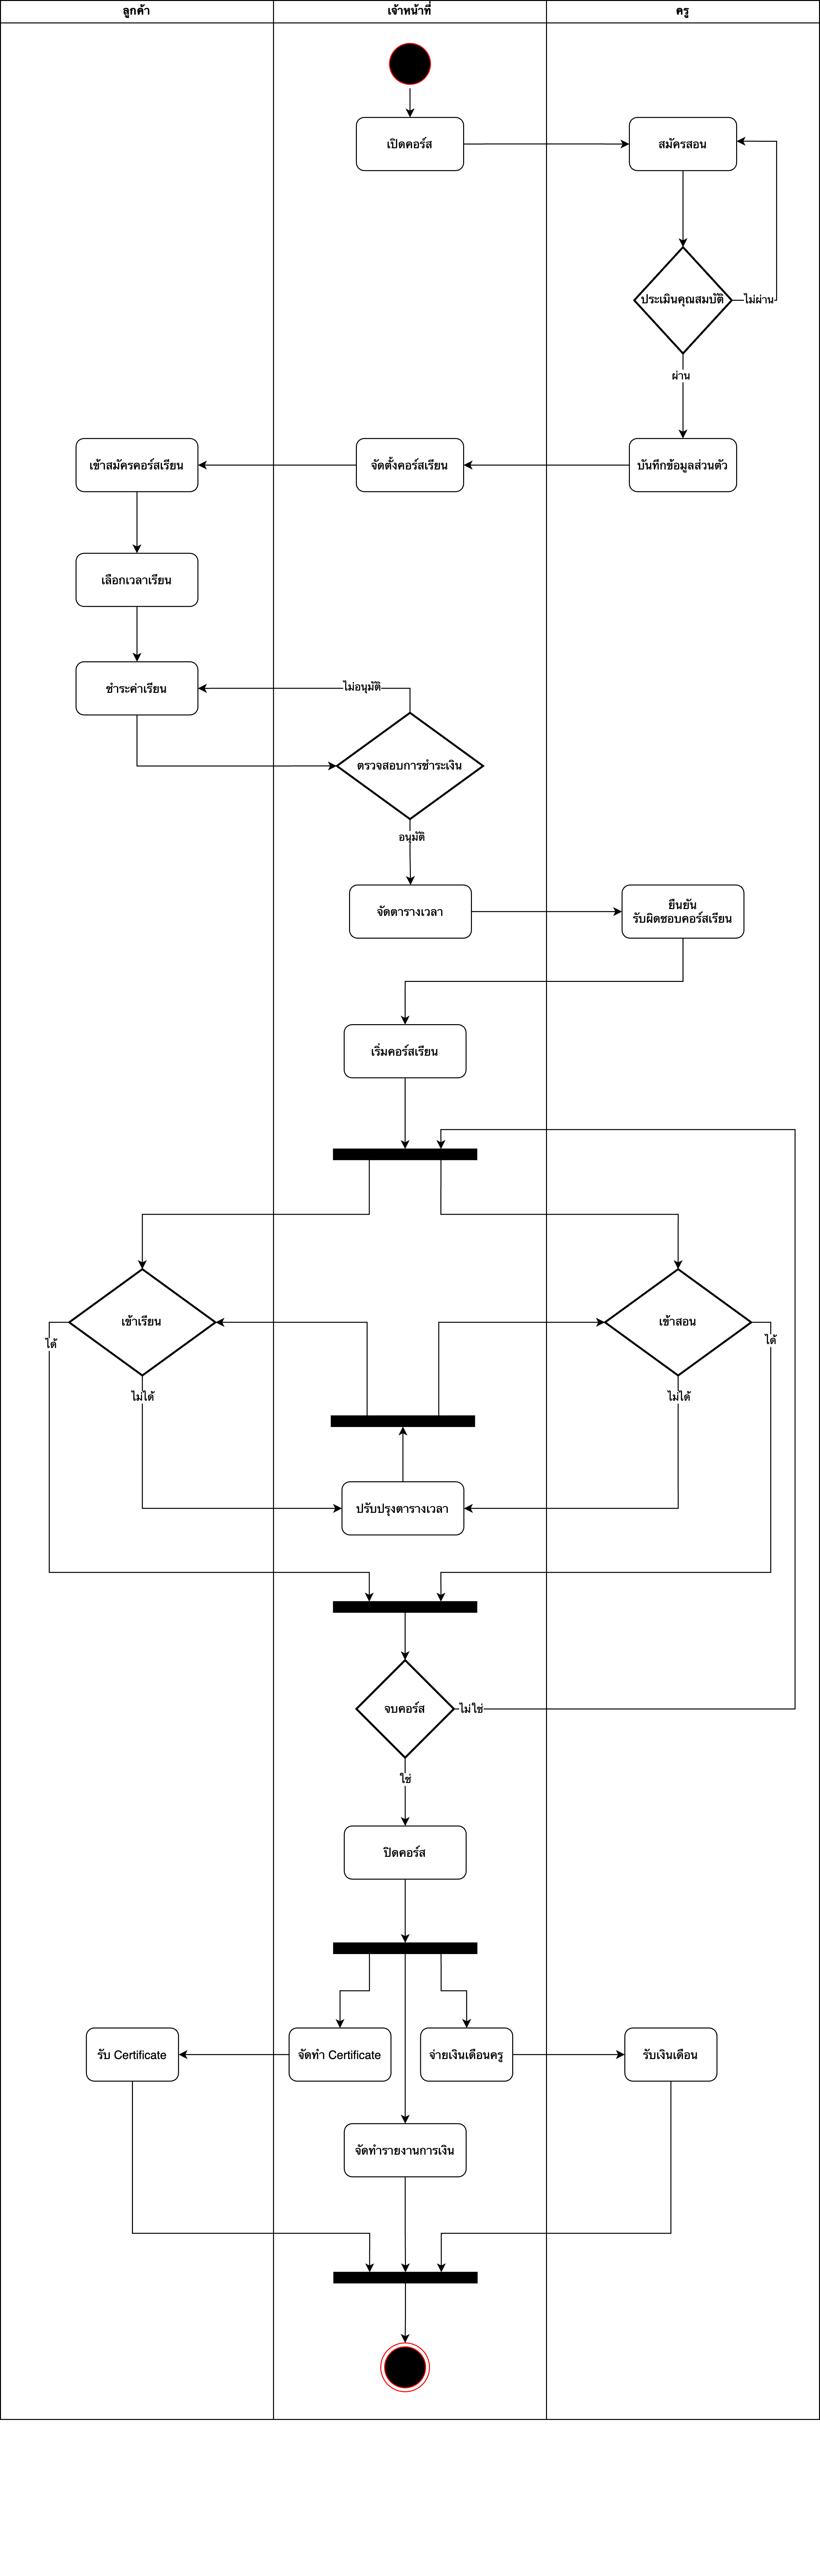
\includegraphics[width=\textwidth]{./images/section-03/aqkids-activities-latest.drawio.png}
\caption{Activity Diagram} \label{fig:aqkids-activities}
\end{figure}

\subsubsection{Business Process ที่สัมพันธ์กับ Use Case}

\subsubsection{ตารางจับคู่ Business ID กับ Use Case ID}

\subsubsection{Use Case Diagram}

\subsubsection{CRUD Table}

\subsubsection{คำอธิบายประกอบ CRUD Table}

\subsubsection{ER Diagram}

\subsubsection{ER Diagram พร้อม MySQL Queries ประกอบ}

\subsubsection{Query Table}

\subsubsection{Table Structure}

\subsubsection{Use Case Descriptions Sequence Diagram และ Collaboration Diagram}

\subsubsection{State Diagram}

\subsubsection{Class Diagram}

\subsubsection{Component Diagram}

\subsubsection{Site Map/User Interface Structure ของ Staff}

\subsubsection{Site Map/User Interface Structure ของ Teacher}

\subsubsection{Site Map/User Interface Structure ของ Student}
